\section{Jakub Mikołajczyk}

Moje zdjęcie: (Zdjęcie: \ref{fig:parrot}).

\begin{figure}[htbp]
    \centering
    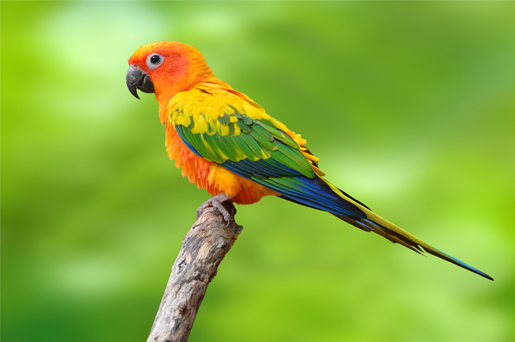
\includegraphics[width=0.3\textwidth]{pictures/jakub.jpg} 
    \caption{To jest papuga}
    \label{fig:parrot}
\end{figure}

Tabela(~\ref{tab:jakub_tabela})

\begin{table}[htbp]\centering
\begin{tabular}{lllll}
\cline{2-5}
\multicolumn{1}{l|}{}      & \multicolumn{1}{l|}{1}    & \multicolumn{1}{l|}{2}    & \multicolumn{1}{l|}{3}    & \multicolumn{1}{l|}{4}    \\ \hline
\multicolumn{1}{|l|}{x}    & \multicolumn{1}{l|}{3 cm} & \multicolumn{1}{l|}{4 cm} & \multicolumn{1}{l|}{5 cm} & \multicolumn{1}{l|}{6 cm} \\ \hline
\multicolumn{1}{|l|}{F(x)} & \multicolumn{1}{l|}{8 N}  & \multicolumn{1}{l|}{15 N} & \multicolumn{1}{l|}{24 N} & \multicolumn{1}{l|}{35 N} \\ \hline
                           &                           &                           &                           &                       


\end{tabular}
\label{tab:jakub_tabela}
\caption{Zależność siły od wychylenia.}
\end{table}

Prawo Ampère'a:
\begin{align}
\oint \vec{B} \cdot d\vec{l} = \mu_0 \cdot I_{\text{enclosed}}
\end{align}

Indukcja:
\begin{itemize}
  \item Prawo Faradaya
  \item Reguła Lenza
  \item Obwód RL
\end{itemize}

Zasady Dynamiki Newtona:
\begin{enumerate}
  \item Pierwsza zasada
  \item Druga zasada
  \item Trzecia zasada
\end{enumerate}



\section*{Nothing twice - Wisława Szymborka}


\begin{center}
\textbf{Nothing} \textit{can ever} \textbf{happen} \textsl{twice.}\\
\textit{In consequence,} \textsl{the sorry fact} \textbf{is}\\
\textsl{that we arrive} \textbf{here improvised}\\
\textit{and leave without} \textbf{the chance to practice.}
\end{center}



